\chapter{Definici� del Projecte}
\label{chapter:definition}
\section{Context}

S'assumeix que es tenen coneixements b�sics d'HTML i d'expressions regulars.

\section{\BibTeX}
\label{chapter:definition:section:bibtex}
Per poder entendre el context del projecte cal que descrivim l'eina de maneig de refer�ncies \BibTeX{} i la sintaxi del llenguatge que utilitza. 
En el nostre cas farem servir aquest llenguatge com a format de sortida al generar els �ndexos bibliogr�fics. Al llistat \ref{listing:exampleBibTeX} es mostra un exemple d'una refer�ncia d'un article cient�fic expressat en el format \BibTeX:
\begin{center}
\begin{lstlisting}[caption={Refer�ncia expressada en \BibTeX}, label=listing:exampleBibTeX]
@article{MoSh:27,
  title = {Size direction games over the real line},
  author = {Moran, Gadi and Shelah, M., Saharon},
  journal = {Israel Journal of Mathematics},
  pages = {442--449},
  volume = {14},
  year = {1973},
}
\end{lstlisting}
\end{center}

Alguns aspectes a comentar sobre l'exemple anterior:
\begin{itemize}
\item{}
La primera l�nia cont� el tipus de document i un identificador. El primer defineix els camps obligatoris que s'han d'especificar, i el segon ens permetr� citar a la refer�ncia des d'un document. En el nostre cas nom�s ens interessen les refer�ncies de tipus \textit{article} i haurem de definir, com a m�nim, els camps \textit{author}, \textit{title}, \textit{journal} i \textit{year}, que s�n obligatoris.

\item{}
Es considera que el nom d'un autor o editor pot constar de quatre parts diferents: \textit{First}, \textit{von}, \textit{Last}, \textit{Jr.}. Es poden ordenar de diverses maneres, per� nosaltres ho farem amb \texttt{<von> <last>, <middle>, <first>}. Cal separar m�ltiples noms amb la paraula \texttt{and}.

\item{}
L'�ltim camp d'una refer�ncia pot acabar o no amb una coma.
\end{itemize}

\section{Funcionalitats}
La llista completa de caracter�stiques del sistema:
\begin{itemize}
\item{}
Extracci� de la refer�ncia bibliogr�fica corresponent a un article d'un fitxer PDF

\item{}
Possibilitat d'exportar les refer�ncies extretes en format \BibTeX{} i desar-les a un fitxer \texttt{.bib}
\end{itemize}


\section{Disseny del sistema}
Hem organitzat el codi del sistema en els m�duls que es llisten a continuaci�:
\begin{itemize}
\item{\textit{Raw Content Extraction} (rce):}
Agrupa totes les classes encarregades d'extreure el contingut dels documents PDF.

\item{\textit{Information Retrieval} (ir):}
Encarregat de comunicar-se amb els diferents cercadors disponibles a Internet per obtenir p�gines que contenen informaci� de la refer�ncia que volem extreure.

\item{\textit{Information Extraction} (ie):}
Cont� tot el codi que permet obtenir la refer�ncia a partir d'una p�gina HTML. A m�s, tamb� �s l'encarregat de generar nous \textit{wrappers}.

\item{\textit{References}:}
Per una banda fa un an�lisis sint�ctic de les refer�ncies extretes per poder-les validar. Per l'altra, transforma a \BibTeX les refer�ncies extretes.

\item{Base de dades (db):}
Tal i com indica el seu nom, duu a terme els accessos la base de dades.

\item{\textit{Main}: }
Enlla�a tots els m�duls anteriors i proporciona punts d'entrada a la interf�cie d'usuari. Fa de fa�ana del sistema.

\item{\textit{Graphical User Interface} (gui):}
Interf�cie d'usuari m�s o menys amigable.
\end{itemize}

La figura \ref{fig:module_diagram} mostra com interaccionen entre ells.

\begin{figure}[h!]
\begin{center}
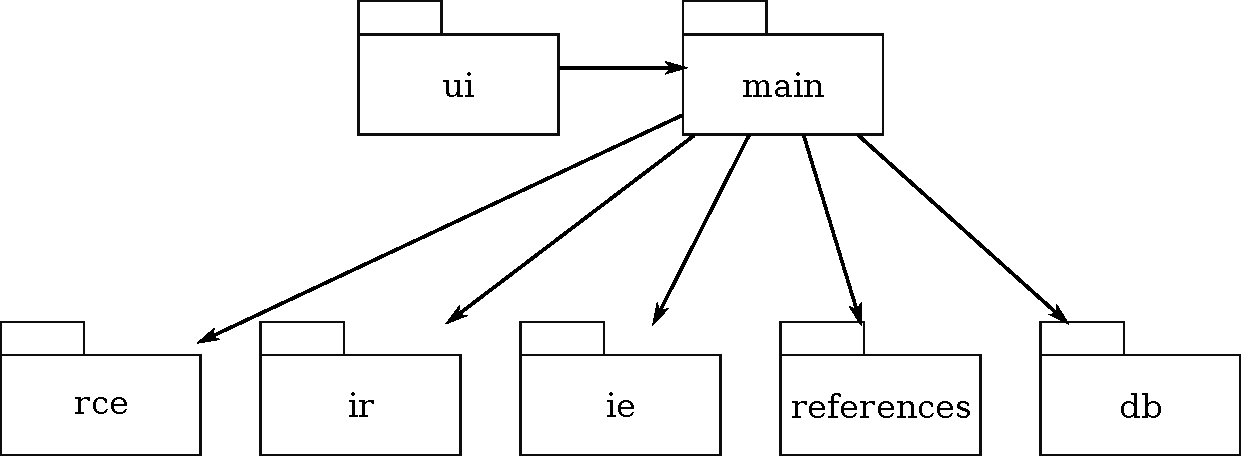
\includegraphics[width=0.6\textwidth]{figures/module_diagram.pdf}
\caption{M�duls del sistema}
\label{fig:module_diagram}
\end{center}
\end{figure}

